\item \textbf{{[}JJC/PRELIM/9597/2018/P2/Q5{]} }

The following shows a message being encrypted using a Caesar cipher.
\begin{center}
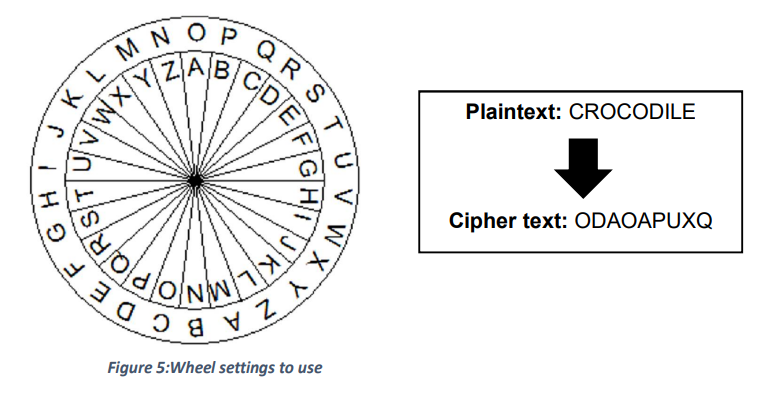
\includegraphics[width=0.5\paperwidth]{C:/Users/Admin/Desktop/Github/question_bank/LyX/static/img/9597-JJC-2018-P2-Q5-1}
\par\end{center}
\begin{enumerate}
\item Decrypt the cipher text \textquotedbl\textbf{QXQBTMZF}\textquotedbl{}
using the Caesar cipher with the settings shown in Figure 5. \hfill{}{[}1{]}
\end{enumerate}
In modern terminology, a Vernam cipher is a symmetrical stream cipher
in which the plaintext is combined with a random or pseudorandom stream
of data (the \textquotedbl keystream\textquotedbl ) of the same
length, to generate the cipher text, using the Boolean \textquotedbl exclusive
or\textquotedbl{} (XOR) function. 
\noindent \begin{center}
\begin{tabular}{|c|c|c|}
\hline 
A & B & A \textbf{XOR} B\tabularnewline
\hline 
0 & 0 & 0\tabularnewline
\hline 
0 & 1 & 1\tabularnewline
\hline 
1 & 0 & 1\tabularnewline
\hline 
1 & 1 & 0\tabularnewline
\hline 
\end{tabular}
\par\end{center}

Using the Vernam cipher method, the plaintext \textquotedbl RUN\textquotedbl{}
is to be encrypted. \textquotedbl RUN\textquotedbl{} will be encoded
using 8-bit ASCII, according to the following ASCII table. 
\noindent \begin{center}
\begin{tabular}{|c|c|c|c|c|c|}
\hline 
Letter & ASCII Code & Letter & ASCII Code & Letter & ASCII Code\tabularnewline
\hline 
A & 01000001 & J & 01001010 & S & 01010011\tabularnewline
\hline 
B & 01000010 & K & 01001011 & T & 01010100\tabularnewline
\hline 
C & 01000011 & L & 01001100 & U & 01010101\tabularnewline
\hline 
D & 01000100 & M & 01001101 & V & 01010110\tabularnewline
\hline 
E & 01000101 & N & 01001110 & W & 01010111\tabularnewline
\hline 
F & 01000110 & O & 01001111 & X & 01011000\tabularnewline
\hline 
G & 01000111 & P & 01010000 & Y & 01011001\tabularnewline
\hline 
H & 01001000 & Q & 01010001 & Z & 01011010\tabularnewline
\hline 
I & 01001001 & R & 01010010 & \multicolumn{1}{c}{} & \multicolumn{1}{c}{}\tabularnewline
\cline{1-4} \cline{2-4} \cline{3-4} \cline{4-4} 
\end{tabular}
\par\end{center}
\begin{enumerate}
\item[(b)]  The key \texttt{10111001} \texttt{01001101} \texttt{01000001} will
be used to perform the encryption. Perform this encryption. Show your
working to derive the cipher text from the plain text. \hfill{}{[}3{]}
\item[(c)]  Both the Caesar and Vernam ciphers are symmetric ciphers. Explain
the difference between a symmetric and an asymmetric cipher system.
\hfill{}{[}1{]}
\end{enumerate}
The following diagram shows the physical topology of a typical home
Local Area Network (LAN) and its connection to the Internet. The LAN
uses the IPv4 protocol. 

Device A is a Wireless Access Point. A range of devices, including
laptop computers and mobile phones connect to the network through
the Wireless Access Point.

Device B is a Network Attached Storage device which is a server used
to store files that can be accessed by other devices connected to
the network. 
\begin{center}
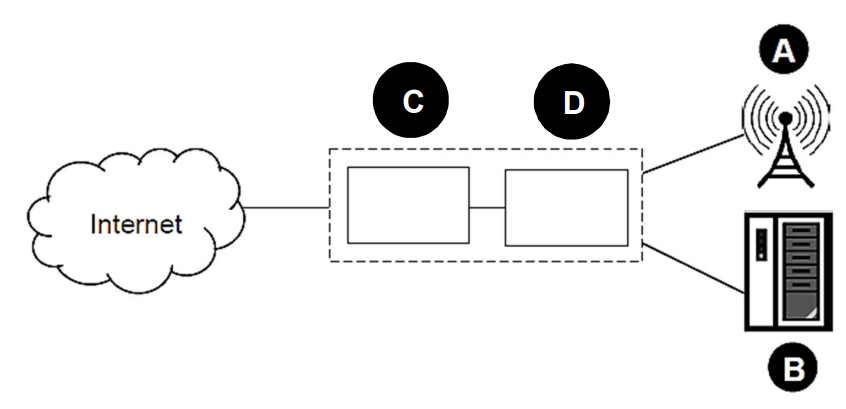
\includegraphics[width=0.5\paperwidth]{C:/Users/Admin/Desktop/Github/question_bank/LyX/static/img/9597-JJC-2018-P2-Q5-2}
\par\end{center}
\begin{enumerate}
\item[(d)]  Identify the two networking devices (C and D). \hfill{}{[}2{]}
\item[(e)]  The devices that are used within the home have private IP addresses.
The Combined Device has both a private IP address and a public IP
address. Explain the differences between private and public IP addresses,
and why the Combined Device has both.\hfill{} {[}3{]}
\item[(f)]  Describe two methods for ensuring the security of access to the
files in Device B. \hfill{}{[}4{]}
\end{enumerate}